\section{JSON}
\begin{frame}
\frametitle{Introducción}
\begin{itemize}
\item	JSON es un formato de intercambio de datos liviano, desarrollado con el objetivo de minimizar el overhead y ser fácilmente legible y editable tanto por máquinas como por seres humanos.
		\pause
\item	Está basado en un subconjunto del estándar de JavaScript, y esto es lo que le da su nombre: ``JavaScript Object Notation''.
\end{itemize}
\end{frame}

\begin{frame}
\frametitle{Un JSON bien formado}
\begin{itemize}
\item	JSON se construye a partir de dos estructuras:
		\pause
\begin{itemize}
		\item	Una colección de pares clave $\rightarrow$ valor (al estilo de un objeto ó record ó struct ó diccionario ó tabla hash ó arreglo asociativo en los lenguajes de programación).
				\pause
		\item	Una lista ordenada de valores (al estilo de un array ó vector ó lista ó secuencia en los lenguajes de programación).
\end{itemize}
\end{itemize}
\end{frame}

\begin{frame}
\frametitle{Un JSON bien formado}
\begin{itemize}
\item	En JSON se representan de las siguientes maneras, respectivamente:
		\pause
\begin{itemize}
		\item	Un objeto comienza con una llave izquierda \texttt{\{} y termina con una llave derecha \texttt{\}}. Cada clave es seguida por dos puntos \texttt{:}, y los pares clave $\rightarrow$ valor se separan mediante una coma \texttt{,}. \\
				\pause
				Gráficamente: \\
				\begin{figure}
				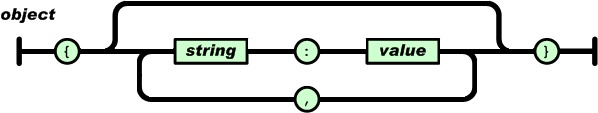
\includegraphics[scale=0.4]{JSONObject}
				\end{figure}
				\pause
		\item	Un arreglo comienza con un corchete izquierdo \texttt{[} y finaliza con un corchete derecho \texttt{]}. Los elementos del arreglo son separados por coma \texttt{,}. \\
				\pause
				Gráficamente: \\
				\begin{figure}
				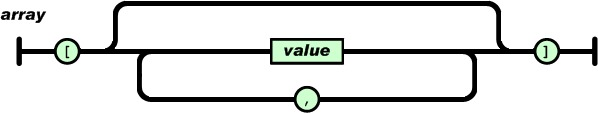
\includegraphics[scale=0.4]{JSONArray}
				\end{figure}
\end{itemize}
\end{itemize}
\end{frame}

\begin{frame}
\frametitle{Un JSON bien formado}
\begin{itemize}
\item	Finalmente, se especifica el tipo de los valores que pueden estar ligados a una clave. Estos son:
\begin{itemize}
	\item	cadenas de texto
	\item	números
	\item	objetos (ítems 'a' de las diapositivas anteriores)
	\item	arreglos (ítems 'b' de las diapositivas anteriores)
	\item	true (literal booleano)
	\item	false (literal booleano)
	\item	null
\end{itemize}
\pause
\item Gráficamente: \\
		\begin{figure}
		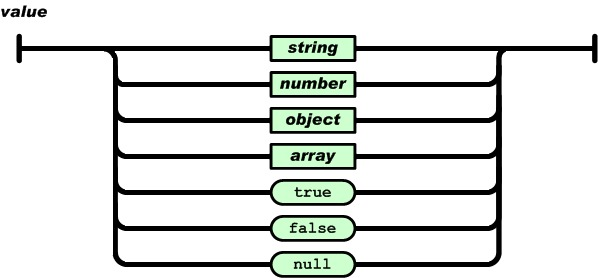
\includegraphics[scale=0.4]{JSONValue}
		\end{figure}
\end{itemize}
\end{frame}

\begin{frame}
\frametitle{JSON vs XML}
\begin{itemize}
\item	JSON se presenta como una alternativa ``fat-free'' a XML, dada la gran diferencia de tamaños entre las codificaciones de un mismo objeto en estos dos formatos. \\
		\pause
\item	Además la lectura y generación de objetos JSON es más simple que las de objetos XML. \\
		\pause
\item	De todos modos, si comprimimos ambas representaciones, por ejemplo, con gzip, la diferencia de tamaños se torna mínima, al ser la compresión muy efectiva ante los repetidos patrones de XML. \\
		\pause
\item	Si además en nuestro dominio es importante contar con el concepto de esquema XML, tipado fuerte y estructura formal con etiquetas predefinidas, entonces es posible que prefiramos aferrarnos a XML antes que utilizar JSON, más allá de su simplicidad y legibilidad.

\end{itemize}
\end{frame}
